% !TEX root = Draft3SM.tex
%======================================================================
% Supplementary Material: computational cost of the formalization.
% Numbers are a lower bound from the local interactive logs
% (generated by the texra-cost-toolkit). All figures are constants defined in
% preamble.tex (\nCost, \nCacheRate, ...). Figures live in figures/cost/ and are
% included at \columnwidth so they cannot overflow; tables from cost_tables.tex.
%======================================================================
\section{Computational cost}\label{app:cost}


The interactive agent runtime recorded a model-API cost of \$\nCost{}, merging
the logs from the two machines used during the project and spanning from
6~February to 29~June 2026. Figure~\ref{fig:cumulative_spend} traces the running
total, in dollars and in tokens. This estimate is approximate: it covers all
model usage in the project workspaces, that is, the full TNLean library rather
than the fundamental theorem alone, and the cost of the headline theorem (in
this case the FT-MPS) cannot be cleanly separated from that of the surrounding
development. It is best read as the cost of building the whole library. A rough
figure for the fundamental theorem alone follows by scaling with code size: the
core chain is about \nLOC{} lines, roughly a quarter of the library, giving an
estimate near \$\nCostFT{}.

\begin{figure}[htbp]
    \centering
    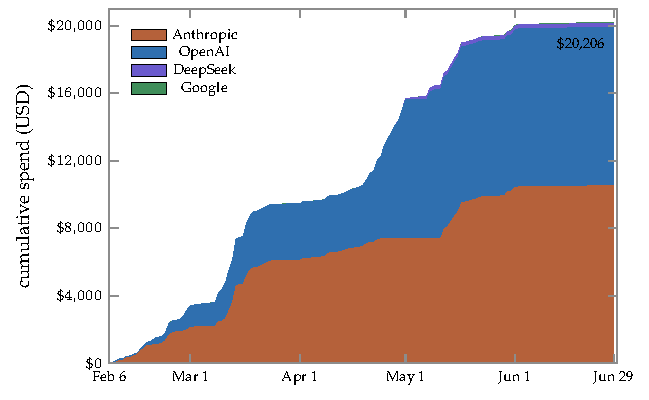
\includegraphics[width=0.49\textwidth]{figures/costs/fig_cumulative_spend.pdf}\hfill
    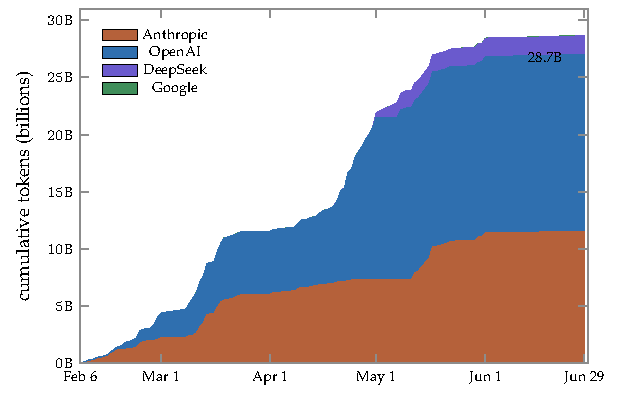
\includegraphics[width=0.49\textwidth]{figures/costs/fig_cumulative_tokens.pdf}
    \caption{Cumulative model-API cost over the development, merging the logs
        from both machines, in dollars (left) and tokens (right). The dollar curve's
        endpoint matches the total quoted in the text, \$\nCost{}; OpenAI and
        DeepSeek account for a larger share of tokens than of cost, since their
        per-token price is lower.}\label{fig:cumulative_spend}
\end{figure}

The cumulative curve has a stepped rather than uniform form, reflecting periods
in which the agents were closing long proof chains or repairing large
dependency breaks. The next breakdown separates the total by agent role.

\begin{figure}[htbp]
    \centering
    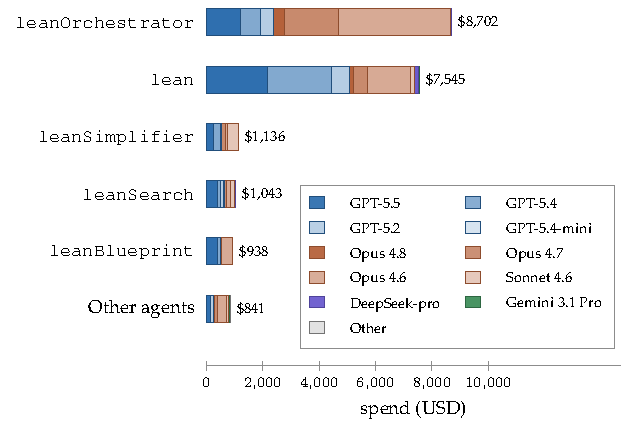
\includegraphics[width=0.49\textwidth]{figures/costs/fig_role_model.pdf}\hfill
    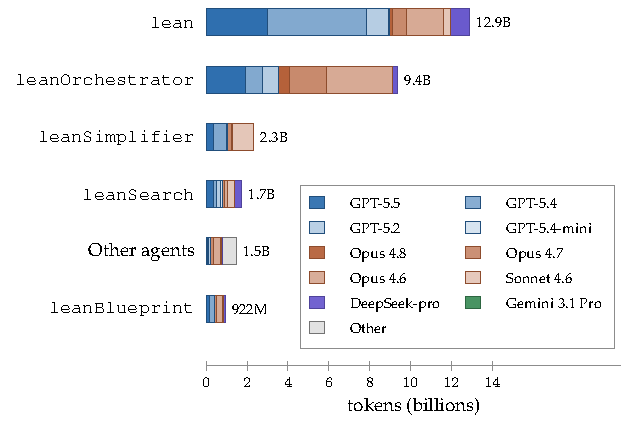
\includegraphics[width=0.49\textwidth]{figures/costs/fig_role_model_tokens.pdf}
    \caption{Cost by agent role, each bar broken down by the language models that
        role used, in dollars (left) and tokens (right). Proof writing and
        orchestration dominate; each provider is shown in one color family.}\label{fig:role_model}
\end{figure}

Proof writing and orchestration together absorbed four fifths of the cost,
consistent with assigning the most capable models to the tasks where an error is
most expensive (\cref{sec:model_selection}). The two roles had different cost
profiles: proof-writing calls had lower average cost but were numerous, whereas
orchestration calls were more expensive because each carried a large context.
Figure~\ref{fig:role_model} breaks each role's cost down by the models it used.
The time-resolved view in \cref{fig:model_gantt} shows when each model was in
use over the project; one panel of each also appears in the End Matter of the
Letter. Each cost figure pairs the dollar view with the same breakdown by
tokens, and the two views do not always agree, since price per token varies
across providers.

\begin{figure}[htbp]
    \centering
    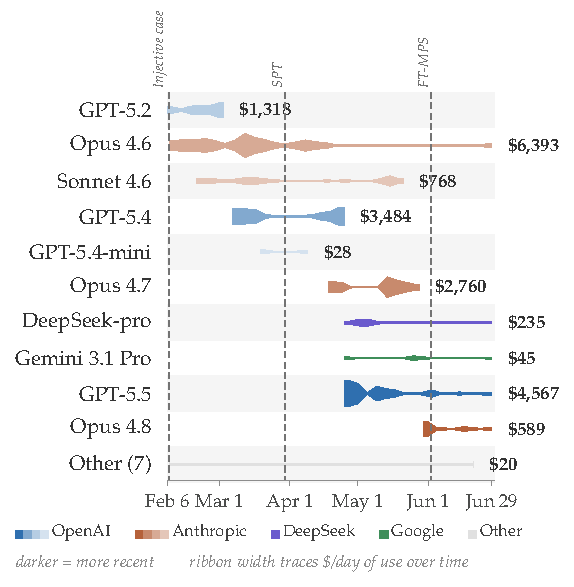
\includegraphics[width=0.49\textwidth]{figures/costs/fig_model_gantt.pdf}\hfill
    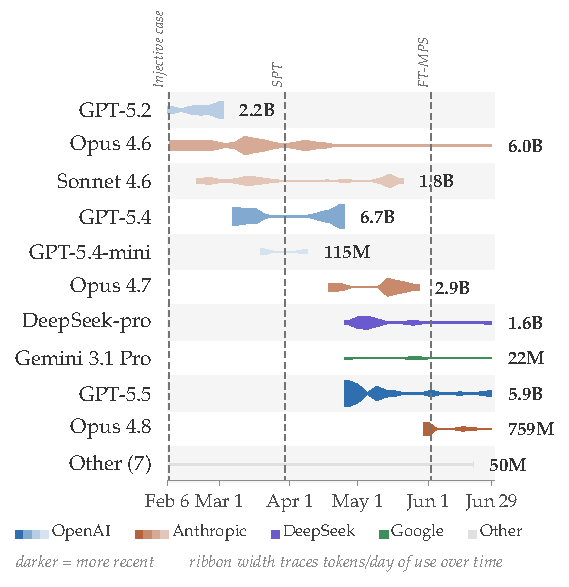
\includegraphics[width=0.49\textwidth]{figures/costs/fig_model_gantt_tokens.pdf}
    \caption{Each model's period of use, sorted by first use and merging both
        machines; one color family per provider, with shade distinguishing models
        within a family. Each ribbon's width traces the intensity of use along its
        own timeline (left: dollars per day; right: tokens per day), on one scale
        shared across every model. Models with less than \$10 of use each are
        grouped into a single ``Other'' row. The dashed vertical
        lines mark the dates the injective case of FT-MPS, the SPT cohomological
        invariant, and the FT-MPS proof chains reported in this work became
        fully verified.}\label{fig:model_gantt}
\end{figure}

The work was split among four providers, with Anthropic and OpenAI together
accounting for 99\% of the metered cost. A portion of the OpenAI work ran
through a code-generation agent on a fixed-price ChatGPT subscription, billed at
\$0 per token but equivalent to about \$\nCodexEq{} at metered API rates (it ran
on GPT-5.4). The same concentration is visible when the data are grouped by
model rather than by role.

\begin{figure}[htbp]
    \centering
    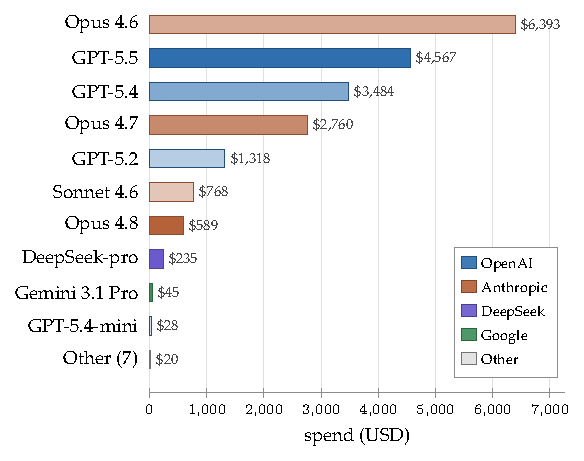
\includegraphics[width=0.49\textwidth]{figures/costs/fig_model_spend.pdf}\hfill
    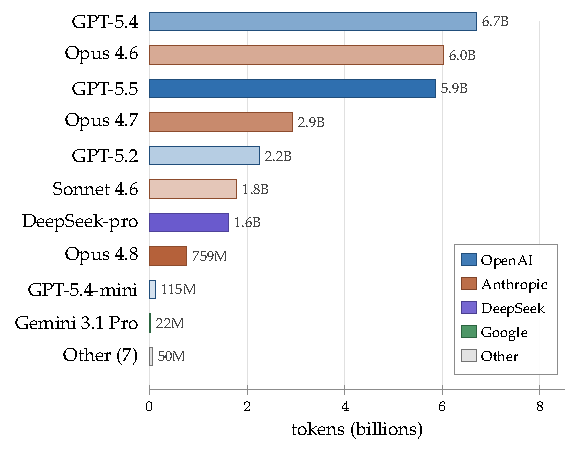
\includegraphics[width=0.49\textwidth]{figures/costs/fig_model_spend_tokens.pdf}
    \caption{Per-model cost over the development, combined across both machines,
        in dollars (left) and tokens (right). The system leaned on a few
        high-capability models for proof writing and orchestration; the less
        expensive models handled high-volume routine work.}\label{fig:model_spend}
\end{figure}

Tables~\ref{tab:cost_model} and~\ref{tab:cost_role} give the numerical
breakdowns by model and role. They should be read with the same caveat as the
figures: the logs cover the interactive runtime for the whole TNLean
development, not only the final FT-MPS proof chain.

% Cost tables - auto-generated (gen_tables.py). Dollars are macros from cost_macros.tex.

\begin{table}[htbp]
    \caption{\label{tab:cost_model}Recorded interactive model-API cost by language model (total $\sim$\$\nCost{} across the development; see text). Input is dominated by cached prompt tokens; OpenAI Codex ran on a ChatGPT subscription, billed at \$0 per token (parenthesized: its equivalent metered cost on GPT-5.4 at the \texttt{llm-zoo} rate \$2.5/\$15 per 1M tokens).}
    \begin{ruledtabular}\begin{tabular}{llrrr}
            Model             & Provider  & Input & Output & Cost (share)                           \\ \colrule
            Claude Opus 4.6   & Anthropic & 6.0B  & 24M    & \$\costMdlClaudeOpusFourSix{} (32\%)   \\
            GPT-5.5           & OpenAI    & 5.8B  & 11M    & \$\costMdlGPTFiveFive{} (23\%)         \\
            GPT-5.4           & OpenAI    & 6.7B  & 21M    & \$\costMdlGPTFiveFour{} (17\%)         \\
            Claude Opus 4.7   & Anthropic & 2.9B  & 9M     & \$\costMdlClaudeOpusFourSeven{} (14\%) \\
            GPT-5.2           & OpenAI    & 2.2B  & 21M    & \$\costMdlGPTFiveTwo{} (7\%)           \\
            Claude Sonnet 4.6 & Anthropic & 1.8B  & 8M     & \$\costMdlClaudeSonnetFourSix{} (4\%)  \\
            Claude Opus 4.8   & Anthropic & 755M  & 4M     & \$\costMdlClaudeOpusFourEight{} (3\%)  \\
            DeepSeek-pro      & DeepSeek  & 1.6B  & 6M     & \$\costMdlDeepSeekpro{} (1\%)          \\
            Gemini 3.1 Pro    & Google    & 22M   & 74k    & \$\costMdlGeminiThreeOnePro{} (0\%)    \\
            GPT-5.4-mini      & OpenAI    & 115M  & 580k   & \$\costMdlGPTFiveFourmini{} (0\%)      \\
            Other models (7)  & ---       & 50M   & 353k   & \$\costMdlOther{} (0\%)                \\
            OpenAI Codex      & OpenAI    & 617M  & 3M     & \$0 ($\approx$\$\nCodexEq{} eq.)       \\
            \colrule
            Total             &           & 28.6B & 108M   & \$\nCost{} (100\%)                     \\
        \end{tabular}
    \end{ruledtabular}
\end{table}

\begin{table}[htbp]
    \caption{\label{tab:cost_role}Recorded cost by agent role. Proof writing and orchestration absorb four-fifths of the cost; orchestration is costly per call because each session carries a large context. Workflow agents run single-pass transformations and make no tool calls, so they are shown separately from the tool-using roles.}
    \begin{ruledtabular}\begin{tabular}{lrrr}
            Role             & Calls   & Cost (share)                     & \$/call                           \\ \colrule
            Orchestrator     & 219     & \$\costRoleOrchestrator{} (43\%) & \$\costRoleOrchestratorPerCall{}  \\
            Proof writer     & 967     & \$\costRoleProofwriter{} (37\%)  & \$\costRoleProofwriterPerCall{}   \\
            Simplifier       & 218     & \$\costRoleSimplifier{} (6\%)    & \$\costRoleSimplifierPerCall{}    \\
            Library scout    & 269     & \$\costRoleLibraryscout{} (5\%)  & \$\costRoleLibraryscoutPerCall{}  \\
            Blueprint sync   & 95      & \$\costRoleBlueprintsync{} (5\%) & \$\costRoleBlueprintsyncPerCall{} \\
            Other tool-using & 486     & \$\costRoleOtherTU{} (3\%)       & \$\costRoleOtherTUPerCall{}       \\
            Workflow agents  & 65      & \$\costRoleWorkflow{} (1\%)      & \$\costRoleWorkflowPerCall{}      \\
            \colrule
            Total            & 2{,}319 & \$\nCost{} (100\%)               &                                   \\
        \end{tabular}
    \end{ruledtabular}
\end{table}


\FloatBarrier

Normalized to output, the cost is about \$\nCostPerKLOC{} per thousand lines of
Lean over the full library. From mid-March onward, separate automated review
agents examined each change proposed to the shared repository and applied fixes;
these agents ran outside the interactive runtime, were billed separately, and
are not included in the \$\nCost{}.
